\chapter{Основные теоретические сведения}
\addcontentsline{toc}{chapter}{Основные теоретические сведения}

\section{Методология ускорения вычислений на основе ПЛИС}

Ускорение вычислительных алгоритмов с использованием программируемых логических интегральных схем (ПЛИС) имеет ряд преимуществ по сравнению с их реализацией на универсальных микропроцессорах, или графических процессорах. В то время, как традиционная разработка программного обеспечения связана с программированием на заранее определенном наборе машинных команд, разработка программируемых устройств - это создание специализированной вычислительной структуры для реализации желаемой функциональности.

На рисунке \ref{png:org_calc} представлены принципы организации вычислений на различных платформах.

\begin{figure}[H]
	\captionsetup{justification=centering}
	\centering{
		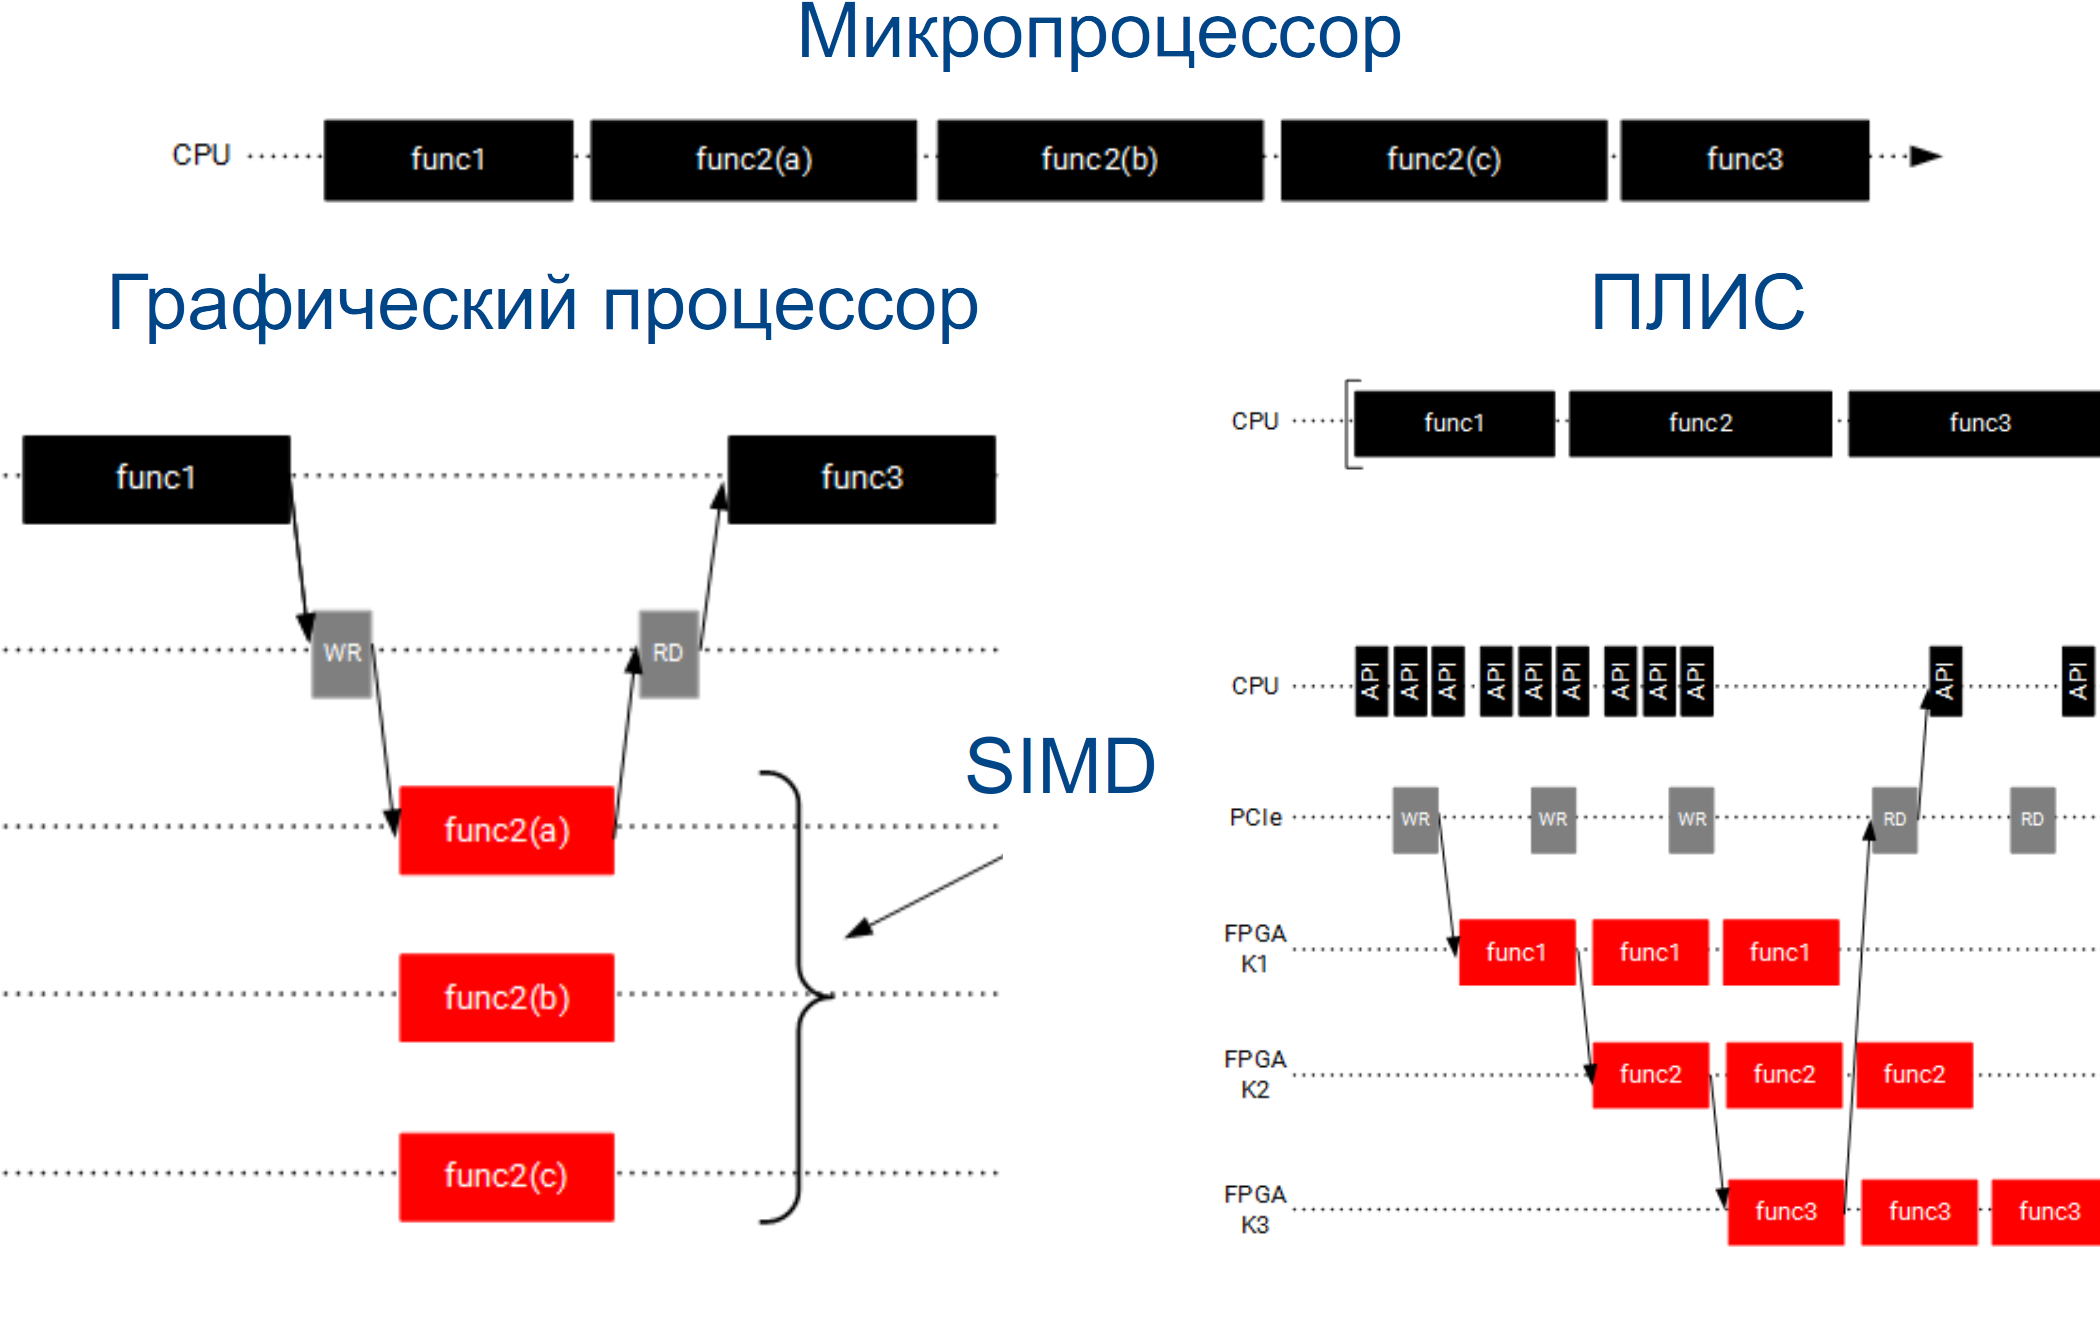
\includegraphics[scale=0.2]{images/org_calc}
		\caption{Принципы организации вычислений на различных платформах}
		\label{png:org_calc}
	}
\end{figure}

Методологию создания ускорителей на ПЛИС с применением средств синтеза высокого уровня (High Level Synthesis, HLS) можно представить в виде трех этапов:
\begin{enumerate}
	\item Создание архитектуры приложения.
	\item Разработка ядра аппаратного ускорителя на языках C/C++.
	\item Анализ производительности и выявление способов ее повышения.
\end{enumerate}


